\chapter{Array Evaluation}
\section{Overview}

\newpage
\section{Mechanical Design}
Mechanical drawings of testarrays

\begin{figure}[h]
	\centering
	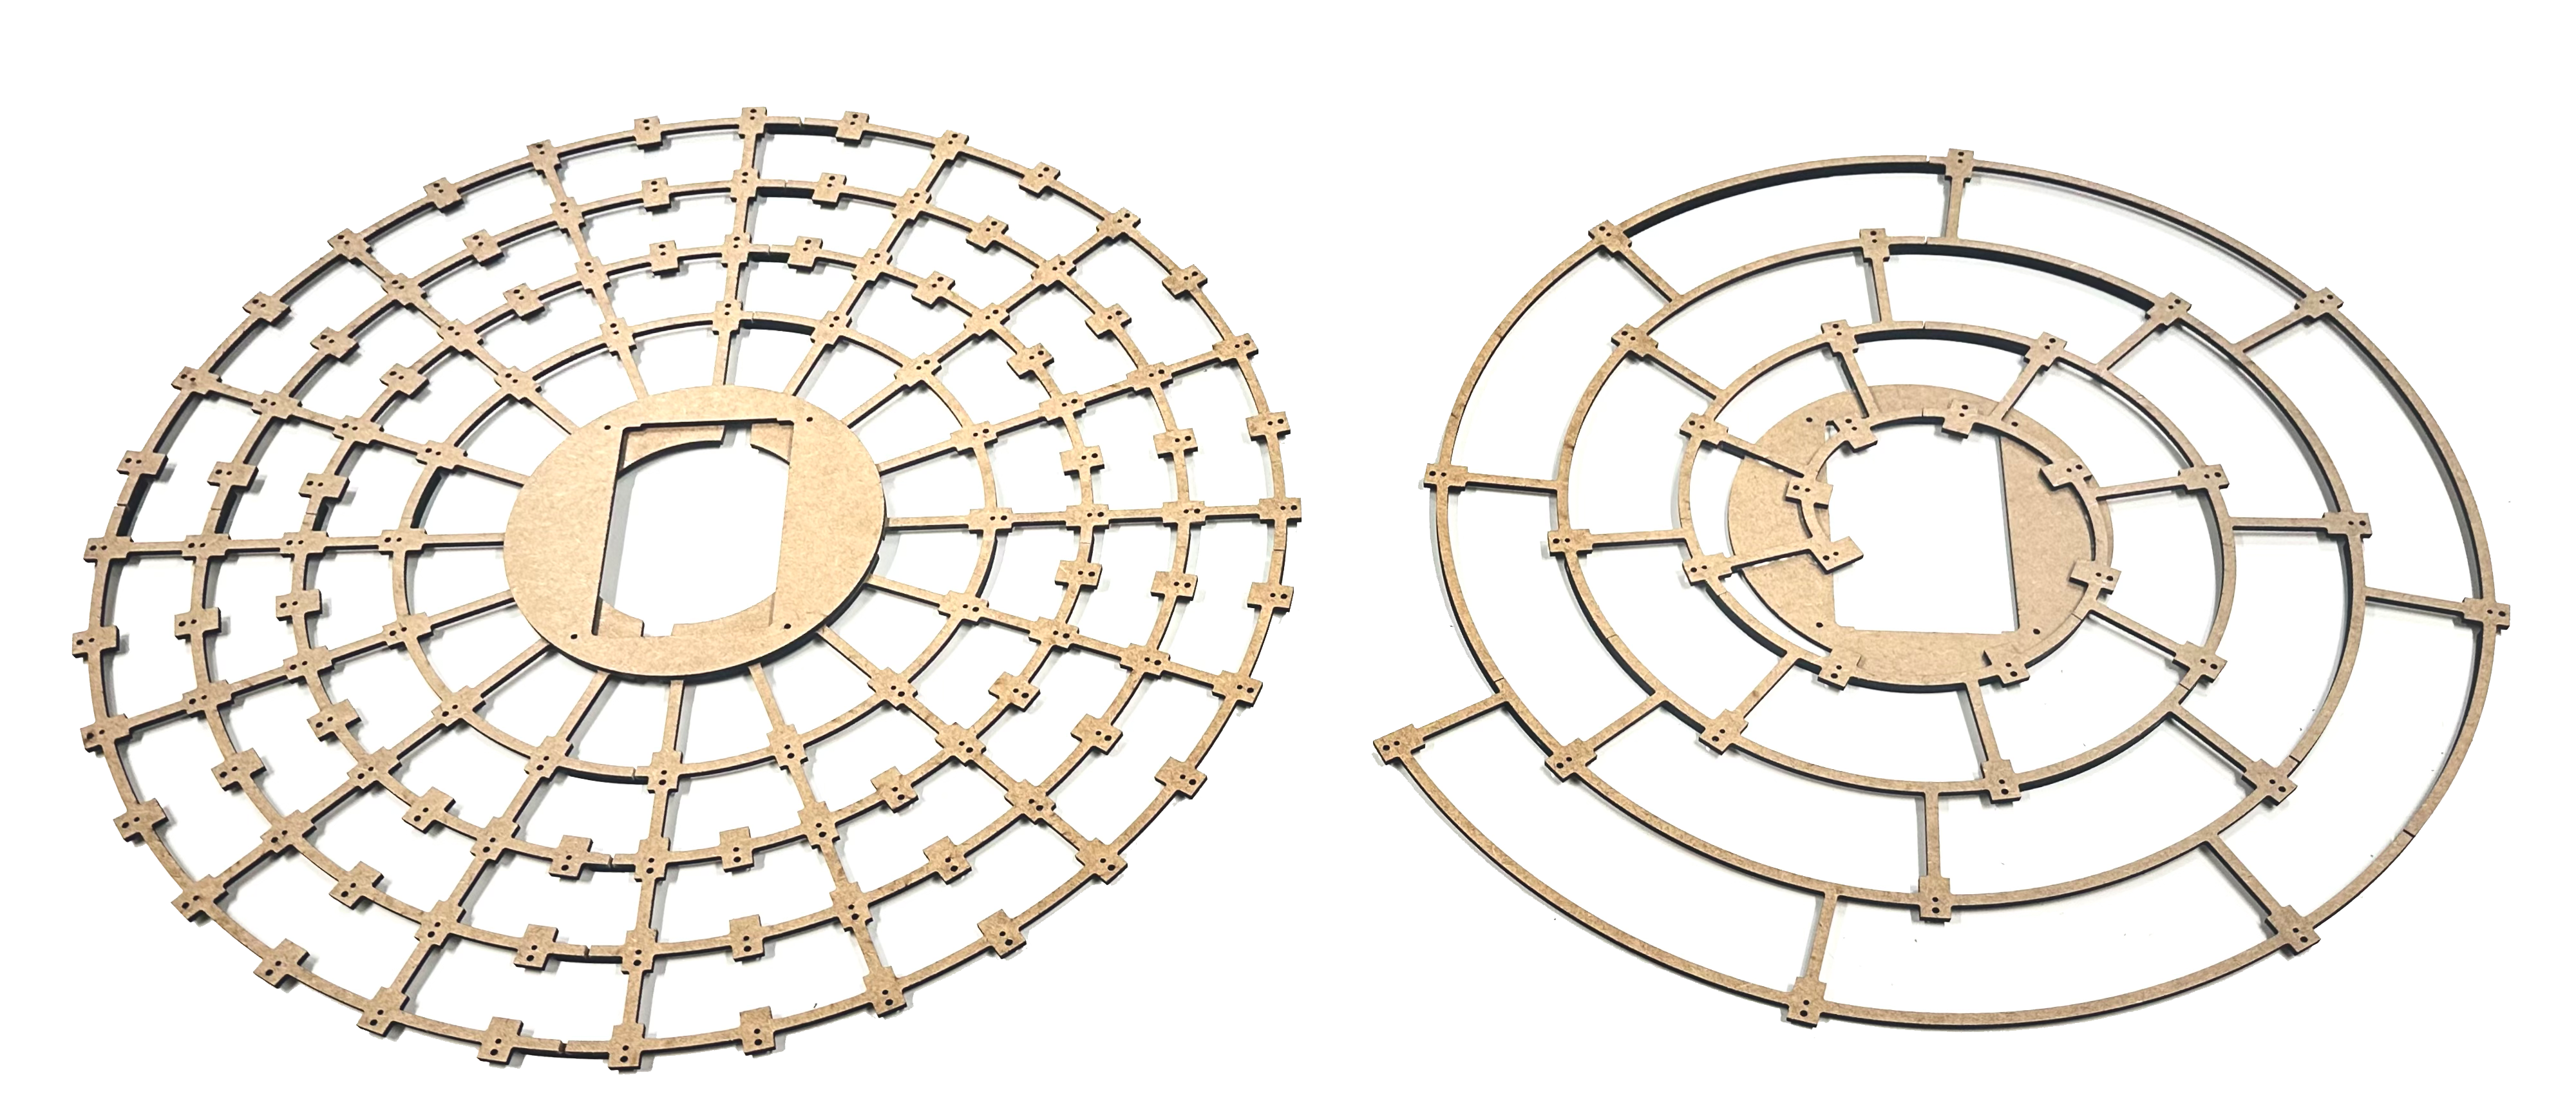
\includegraphics[width=1.0\textwidth]{images/5_array_evaluation/wooden_arrays.png}
	\caption{Wooden Prototype Arrays (Left: Circular Array, Right: Archimedean Spiral Array)}
	\label{fig:wooden_arrays}
\end{figure}

\newpage
\section{Metrics}
TO evaluate the performance of an array several metrics are used.
In \todo{Cite Array design s40430-018-1275-5-1, array design comparisons} the
main beam-width is proposed.
\todo{cite Circ array drone trackings13638-019-1632-9} is using the ratio
between the main lobe power and the side lobe power.
Another measure related to the main lobe with is the main lobe area.
The main lobe is defined as all the points around the peak where their value
is greater than half the peaks value. \todo{besser englisch}

Blabla

\newpage
\section{Measurements \& Findings}
Blabla


\newpage
\section{Conclusion}
Blabla
